\section{Introduction}
\vspace{-3mm}

Recent advances in large language models (LLMs) have unlocked remarkable reasoning capabilities, largely driven by reinforcement learning (RL) from outcome-based feedback. By fine-tuning models to maximize verifiable rewards, LLMs like DeepSeek-R1~\citep{guo2025deepseek} and SimpleRL~\citep{zeng2025simplerl} have demonstrated sophisticated behaviors in self-correction and multi-step deduction.

A complementary line of work augments LLMs with external tools (e.g., web search, code execution) for knowledge retrieval and precise computation. Tool-integrated reasoning (TIR) extends reinforcement learning with verifiable rewards to learn \emph{when} and \emph{how} to call tools by interleaving reasoning (e.g., \texttt{<think>}) with tool invocations (e.g., \texttt{<tool\rule[0ex]{0.5em}{0.1pt}call>}) under full context~\citep{jin2025search, song2025r1, chen2025research, feng2025retool}. Early systems supported only a single tool type, whereas recent work enables multi-tool settings by encoding tool metadata into prompts~\citep{dong2025tool, qian2025toolrl, zhang2025nemotron}. However, these methods still train a \emph{single}, monolithic policy under multi-turn full-context reasoning, which introduces scaling challenges: (i) \emph{training} becomes increasingly unstable as horizons lengthen, tool diversity grows, and environments shift with tool feedback~\citep{wang2025ragen, mai2025agent, Moonshot2025KimiResearcher, xue2025simpletir}; and (ii) \emph{inference}-time generalization remains brittle to unseen tasks or tools~\citep{dong2025tool, hu2025owl}.

Agentic systems~\citep{wu2024autogen,hong2024metagpt,hu2025owl} offer a promising alternative to monolithic tool-integrated reasoning models. They consist of multiple modules—often distinct LLMs with prescribed roles (e.g., planner, critic) or specialized components with dedicated tools and capabilities (e.g., executor, coder)—that coordinate via shared memory and inter-module communication. By decomposing problems into sub-goals and iterating over multiple turns, these systems can tackle tasks that demand diverse tools, long horizons, or multi-stage reasoning. However, achieving robust coordination in such systems ultimately requires \emph{training}, since handcrafted logic or static prompting cannot reliably capture when and how modules should collaborate, adapt to evolving tool outputs, or recover from early mistakes. At the same time, they introduce new \emph{training} challenges: modules coordinate sequentially, outcome feedback propagates through long reasoning chains, and state distributions shift with evolving tool outputs. As a result, most systems remain \emph{training-free}, relying on handcrafted logic or prompting heuristics. While some employ supervised fine-tuning or preference optimization for key modules~\citep{motwani2024malt, park2025maporl}, these off-policy approaches are decoupled from live dynamics and learn poorly from downstream successes or failures. Thus, agentic systems struggle with sparse rewards, brittle adaptation, and inefficient orchestration in dynamic environments.



To address the central challenge of learning long-horizon reasoning with sparse rewards in tool-integrated agentic systems, we introduce \model, a \emph{trainable} framework for effective planning and tool use (Figure~\ref{fig:agentflow}). \model comprises four specialized modules—planner, executor, verifier, and generator—that interact iteratively over multiple turns via a shared evolving memory and a toolset. The system operates \emph{in the flow}, with each turn cycling through planning, execution, and verification. Unlike prior agentic systems, \model directly optimizes its planner on-policy, \emph{inside} the live multi-turn loop, allowing it to dynamically adapt to trajectories shaped by tool calls, verifier signals, and memory updates. This evolving memory serves as a deterministic, structured record of the reasoning process, enabling transparent state tracking, controllable behavior, and bounded context growth.



\begin{figure}[t!]
    \centering
    \vspace{-5mm}
    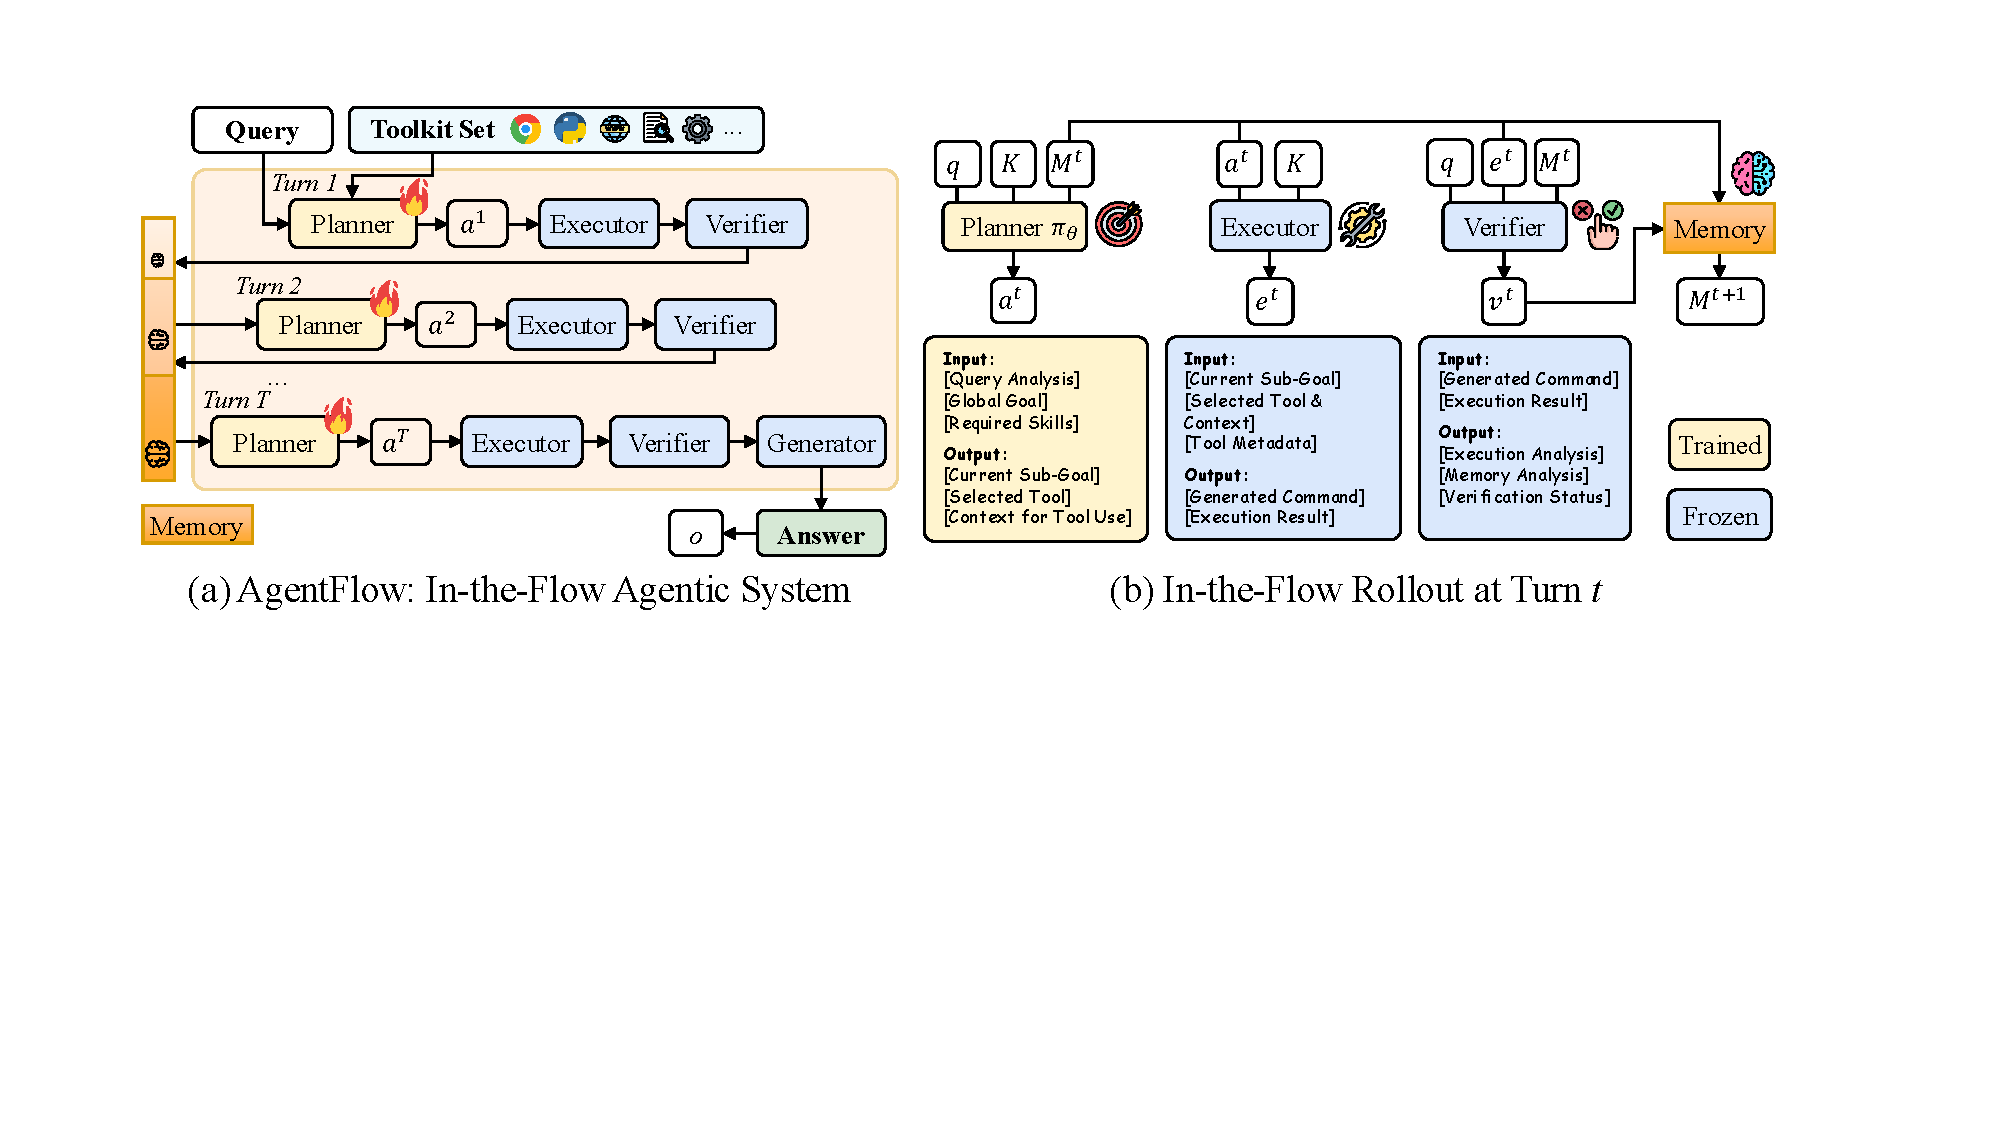
\includegraphics[width=1\linewidth]{figs/fig2_preliminary.pdf}
    \vspace{-5mm}
    \caption{\textbf{(a)} Overview of \model, a trainable agentic system for in-the-flow planning and tool use. Four modules (\text{planner}, \text{executor}, \text{verifier}, \text{generator}) coordinate via a shared evolving memory $M$ and toolset $K$, given a query $q$. The planner policy is optimized on-policy \emph{inside} the system's multi-turn loop to enable adaptive, long-horizon reasoning. \textbf{(b)} A single state transition, showing the action $a^t$, execution result $e^t$, and verifier signal $v^t$ that update the memory from $M^t$ to $M^{t+1}$.}
    \vspace{-6mm}
    \label{fig:agentflow}
\end{figure}

To train the planner on-policy within this agentic system, we need to overcome the long-horizon credit assignment problem inherent to sparse, trajectory-level rewards. We introduce \emph{Flow-based Group Refined Policy Optimization} (Flow-GRPO, Figure~\ref{fig:flow-grpo}), an on-policy algorithm designed for this setting. Flow-GRPO operates on \emph{in-the-flow} rollouts, which capture the full trajectory of states, actions, and tool events induced by the live system. Instead of attempting to assign credit with brittle, intermediate heuristics, we assign a single, verifiable final-outcome reward to the entire trajectory and \emph{broadcast} it to every turn. This design effectively transforms the multi-turn reinforcement learning challenge into a series of single-turn updates: at each turn, the planner has access to the full memory context and receives a consistent reward signal aligned with global success. This approach, coupled with group-normalized advantages to stabilize training, enables robust credit assignment and allows the planner to learn effective long-horizon strategies from sparse feedback.


We evaluate \model on ten benchmarks across diverse reasoning domains, as results highlighted in Figure~\ref{fig:teaser_main_scores}.
\model substantially outperforms top-performing specialized tool-integrated reasoning models and agentic systems, achieving average accuracy by 14.9\% on knowledge-intensive search, 14.0\% on broader agentic tasks, 14.5\% on mathematical reasoning, and 4.1\% on scientific reasoning (\S\ref{subsec:main_results}). 
Notably, our 7B-backbone system even surpasses the $\sim$200B-parameter GPT-4o ~\citep{hurst2024gpt} across all domains. Further analyses confirm that our in-the-flow optimization with Flow-GRPO is crucial, far surpassing offline supervised tuning (\S\ref{subsec:training_planner}). The trained planner learns to optimize planning, enhance tool-calling reliability, and discover effective solution pathways (\S\ref{subsec:optimized_planning}). Moreover, our training approach proves highly efficient, leading to increased rewards and condensed responses compared to traditional tool-integrated RL methods (\S\ref{subsec:traing_efficency}). Finally, we demonstrate that these benefits generalize, with consistent gains from scaling backbone size and turn budget (\S\ref{subsec:scaling_trends}).

Our work makes three key contributions: 
(1) We present \model, a trainable \emph{in-the-flow} agentic system that directly optimizes its planner \emph{inside} the multi-turn loop. By coordinating specialized modules through an evolving memory, it enables adaptive long-horizon planning and robust tool orchestration.
(2) We introduce \emph{Flow-GRPO}, an on-policy, outcome-driven algorithm that hat \emph{converts} multi-turn RL into a sequence of tractable \emph{single-turn} policy updates by \emph{broadcasting} a single, verifiable final-outcome reward to every turn.
(3) Through comprehensive experiments on ten benchmarks, we show that \model with a 7B backbone outperforms specialized baselines and even larger proprietary models. Further analyses reveal improved planning, enhanced tool-calling reliability, and positive scaling with model size and turn budgets.

\vspace{-2mm}
\section{Preliminary}
\label{sec:preliminary}
\vspace{-1mm}

\paragraph{Reinforcement learning for reasoning LLMs.}
Recent progress in reasoning LLMs has been significantly driven by reinforcement learning from outcome feedback, using a verifiable reward signal~\citep{shao2024deepseekmath, yu2025dapo}. 
This paradigm fine-tunes a language model to maximize an outcome-based reward while remaining close to a reference policy. 
Formally, the objective is to optimize a policy LLM $\pi_\theta$\textbf{} to generate a response $o$ for a given query $q$ from dataset $\mathcal{D}$:
\vspace{-1mm}
\begin{equation}
    \label{eq:rl_obj}
    \max_{\pi_\theta} \; \mathbb{E}_{q \sim \mathcal{D}, \, o \sim \pi_\theta(\cdot \mid q)} 
    \big[ R(q, o) \big] 
    - \beta \, \mathbb{D}_{\text{KL}} \!\left( \pi_\theta(o \mid q) \,\|\, \pi_{\text{ref}}(o \mid q) \right),
\end{equation}
where $R(q, o)$ is the outcome-based reward, $\pi_{\text{ref}}$ is a reference model to prevent policy collapse, and $\beta$ controls KL regularization. Algorithms like Group Relative Policy Optimization (GRPO)~\citep{shao2024deepseekmath} implement this by sampling groups of responses, normalizing advantages by their rewards, and updating the policy with a clipped objective to encourage high-reward outputs.

\begin{figure}[th!]
    \centering
    \vspace{-7mm}
    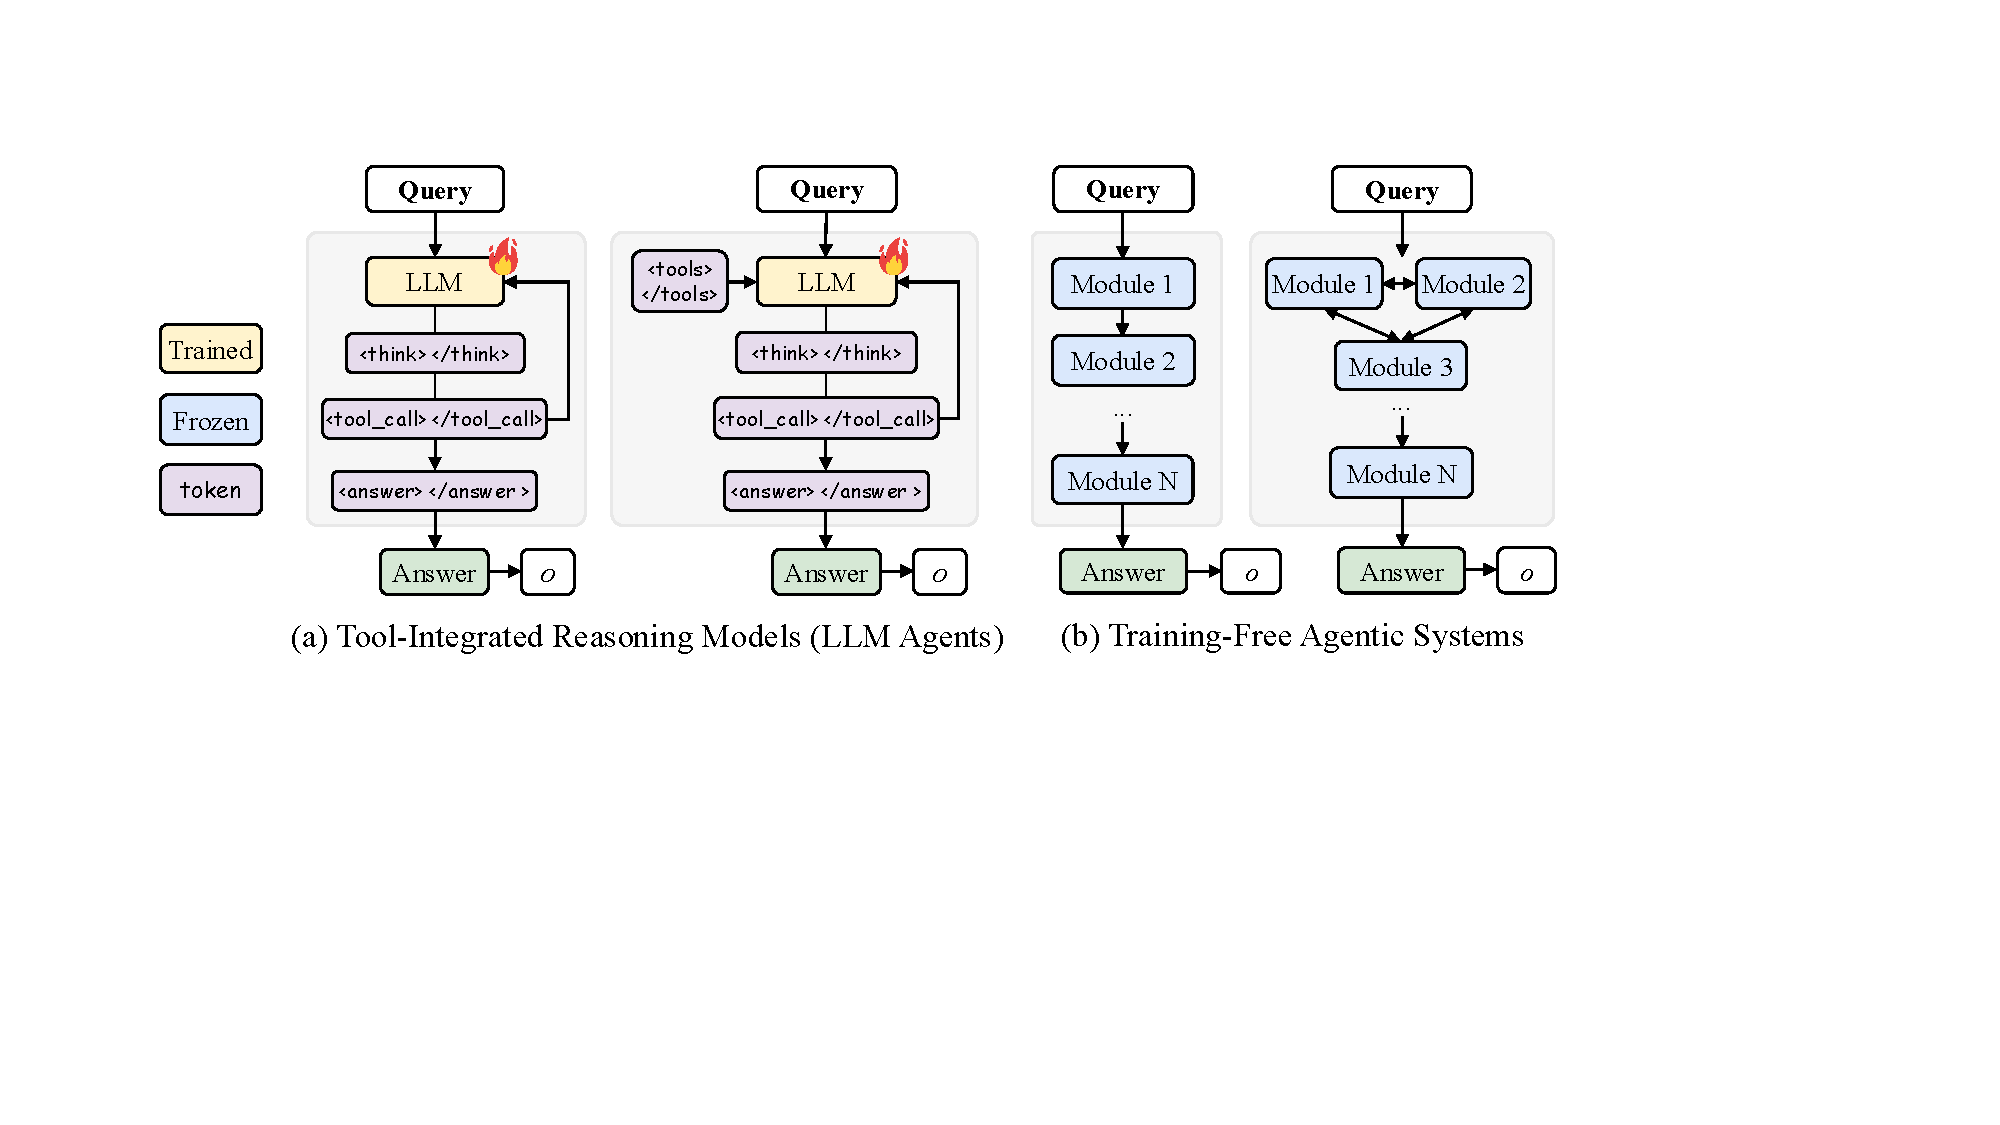
\includegraphics[width=1.0\linewidth]{figs/app_fig_preliminary.pdf}
    \vspace{-5mm}
    \caption{\textbf{Comparison of two paradigms of LLMs with tool use.} (a) Monolithic tool-integrated reasoning models train a single policy to interleave reasoning (e.g., \texttt{<think>}) and tool calls (e.g., \texttt{<tool\_call>}) within a single, full-context trajectory. (b) Agentic systems decompose tasks across multiple specialized modules (e.g., planner, coder) that collaborate. These systems are typically training-free, orchestrated by handcrafted logic or prompting.}
    \label{fig:app_preliminary}
    \vspace{-4mm}
\end{figure}

\paragraph{Tool-integrated reasoning models (LLM agents).}
LLMs can be augmented with external tools to access knowledge and perform precise computation under reinforcement learning with outcome-based reward. As shown in Figure~\ref{fig:app_preliminary}(a), the LLM \emph{interleaves} reasoning and tool calls,  producing a chain of thought within \texttt{<think></think>} tokens followed by tool invocations (e.g., \texttt{<tool\rule[0ex]{0.5em}{0.1pt}call></tool\rule[0ex]{0.5em}{0.1pt}call>}). The resulting trajectory $\tau$ is a sequence of model generations and tool observations: $\tau = \{s^1, a^1, e^1, \ldots, s^T, a^T\}$, where $s^t$ denotes the context, $a^t$ the generated action (thought + tool call), and $e^t$ the tool’s execution result. The policy model $\pi_\theta$ is then trained to maximize a final outcome reward. Prior work has explored single- and multi-tool settings for search and code execution \citep{jin2025search, chen2025research, feng2025retool, qian2025toolrl}.

\paragraph{Agentic systems with tool usage.}
An alternative approach is the use of agentic systems~\citep{wu2024autogen,hong2024metagpt,lu2025octotools}. As shown in Figure~\ref{fig:app_preliminary}(b), these frameworks deploy multiple specialized modules—often distinct LLMs with carefully designed prompts and roles—within a collaborative workflow. By decomposing tasks and assigning subproblems to modules with dedicated tools and capabilities (e.g., planner, coder, critic), they can address complex problems such as web browsing, document processing, and multi-stage programming that exceed the scope of a single model. A central limitation, however, is that these systems are typically \textit{training-free}: modules remain frozen pre-trained models orchestrated by handcrafted logic or prompting heuristics.


\vspace{-1mm}
\section{In-the-Flow Agentic System Optimization}
\label{sec:methodology}
\vspace{-1mm}

We aim to bridge the gap between trainable but monolithic reasoning models and flexible yet static agentic systems. We present \model, a flexible and trainable agentic system that integrates four specialized modules with an evolving memory (\S\ref{subsec:agentflow}). 
Unlike prior agentic systems, \model directly optimizes the planner \emph{within} the multi-turn loop of an agentic system (\S\ref{subsec:flow-grpo}).



\vspace{-1mm}
\subsection{\model: An In-the-Flow Agentic System}
\label{subsec:agentflow}


We propose \model, a general-purpose tool-integrated agentic framework for solving complex reasoning tasks through fine-grained planning and effective tool use within a multi-turn architecture. As shown in Figure~\ref{fig:agentflow}, the framework comprises four specialized modules—\textbf{Action Planner} $\mathcal{P}$, \textbf{Tool Executor} $\mathcal{E}$, \textbf{Execution Verifier} $\mathcal{V}$, and \textbf{Solution Generator} $\mathcal{G}$—coordinated by a shared evolving memory $M$ and a toolset $K$. These modules interact sequentially and iteratively to perform \emph{action planning}, \emph{tool execution}, \emph{context verification}, and \emph{solution generation}, thereby enabling tool-integrated reasoning across multiple turns.


We formalize \model's problem-solving process as a multi-turn Markov Decision Process (MDP). Given a query $q$ and a toolset $K$, the system proceeds for a variable number of turns. Let $M^t$ denote the memory state before turn $t$ (with $M^1$ initialized from $q$). At turn $t$, the planner $\mathcal{P}$ (a trainable policy $\pi_\theta$) formulates a sub-goal, selects an appropriate tool $k \in K$, and retrieves relevant context from memory, producing an action: $a^t \sim \pi_\theta(a^t \mid q, K, M^t)$.


The executor $\mathcal{E}$ invokes the chosen tool with context, yielding an execution observation $e^t \sim \mathcal{E}(e^t \mid a^t, K)$.
The verifier $\mathcal{V}$ then evaluates whether $e^t$ is valid and whether the accumulated memory is sufficient to solve the query, producing a binary verification signal $v^t \sim \mathcal{V}(v^t \mid q, e^t, M^t)$.
If $v^t = 0$, the memory is updated deterministically to incorporate new evidence: $M^{t+1} = f_{\text{mem}}\!(M^t, a^t, e^t, v^t)$,
where $f_{\text{mem}}(\cdot)$ denotes the memory-update function, which records agent-process information in a concise, structured form along with contextual details such as time, turn index, and error signals.

The process repeats until $v^t = 1$ (termination) or a predefined maximum turn budget is reached. Upon termination at turn $T$, the solution generator $\mathcal{G}$ produces the final solution $o$, conditioned on the query and the accumulated memory: $o \sim \mathcal{G}(o \mid q, M^T)$.

This formulation decomposes multi-turn, tool-integrated reasoning into structured, observable transitions. After $T$ turns, the trajectory $\tau = \{(a^t, e^t, v^t)\}_{t=1}^T$ records the history of planning, execution, and verification. The joint generative process can be written as
\vspace{-1mm}
{\small
\begin{equation}
    \label{eq:joint_policy}
    p_\theta\!\left(\{a^t, e^t, v^t\}_{t=1}^T,\, o \mid q, K\right)
    = \Bigg[\prod_{t=1}^T \pi_\theta(a^t \mid q, K, M^t)\;
      \mathcal{E}(e^t \mid a^t, K)\;
      \mathcal{V}(v^t \mid q, e^t, M^t)\Bigg]\;
      \mathcal{G}(o \mid q, M^T),
\end{equation}
}where $\{a^t, e^t, v^t\}_{t=1}^T$ are explicit realizations of the latent reasoning chain. Importantly, unlike latent thoughts behind trajectories, our memory $M$ is an explicit and deterministic record of the reasoning process, ensuring transparency and controllability of multi-turn decisions.

\begin{figure}[t!]
    \centering
    \vspace{-2mm}
    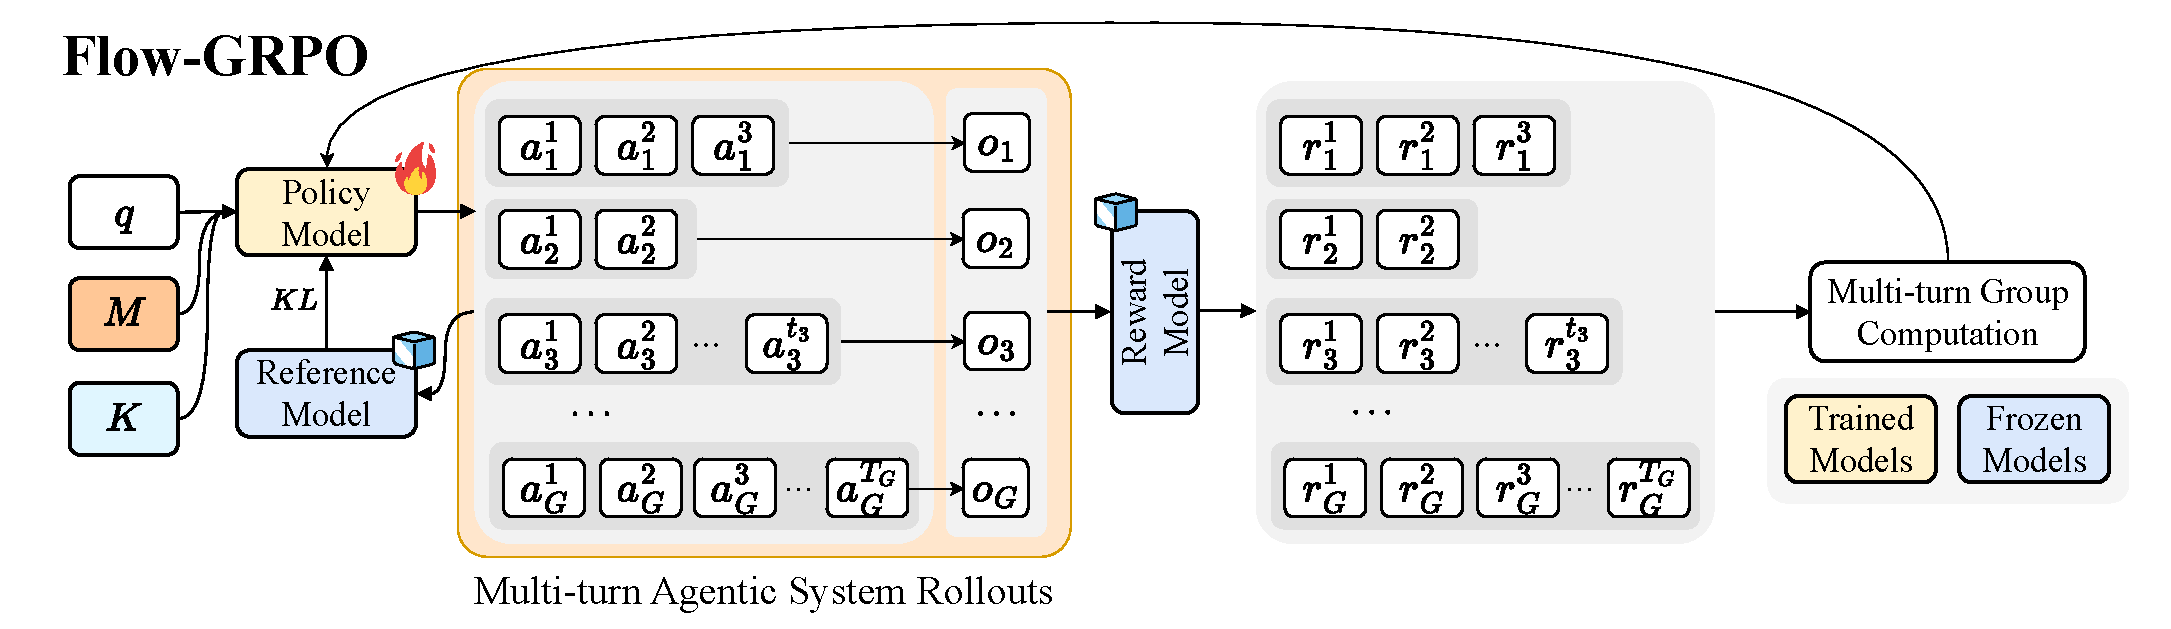
\includegraphics[width=0.95\linewidth]{figs/fig3_method.pdf}
    \vspace{-2mm}
    \caption{\textbf{Optimization for our proposed agentic system \model.} Given a query $q$, an evolving memory $M$, and a toolset $K$, the policy model generates actions that target sub-goals and select tools. It is trained via \textit{Flow-based Group Refined Policy Optimization} (Flow-GRPO), which enables multi-turn reinforcement learning and stable optimization under collaborative dynamics.}
    \vspace{-4mm}
    \label{fig:flow-grpo}
\end{figure}

\vspace{-1mm}
\subsection{In-The-Flow Reinforcement Learning Optimization}
\label{subsec:flow-grpo}
 
We target tool-integrated \emph{agentic systems} operating under \emph{long-horizon} tasks with \emph{sparse} rewards. In this setting, the \textbf{Action Planner} (the trainable policy of \model) selects a \emph{sequence} of interdependent actions while the state $(q, K, M^t)$ evolves with tool results and verifier feedback. Conventional \textit{offline} training—e.g., supervised fine-tuning or preference fine-tuning on curated traces—optimizes the planner \emph{outside} the active loop~\citep{motwani2024malt, park2025maporl}. This decoupling prevents real-time coordination with the executor, verifier, and solution generator, induces distribution shift between training and deployment, and provides limited guidance about \emph{which} intermediate decisions truly matter. As a result, planners often adapt poorly to multi-turn dynamics; early errors cascade, and post-hoc fixes are brittle.

\paragraph{In-the-flow learning.}
To address these issues, we optimize the planner \emph{in the flow} of execution. We roll out the full \model system under the current policy, collect the actual trajectory $\tau$ of states, actions, and tool events it induces, and update the policy within the agentic system using a verifiable final-outcome signal. This exposes the multi-turn credit-assignment problem directly and trains the planner on the exact states it will face at inference. Our objective, Flow-GRPO, is designed to stabilize learning under sparse, trajectory-level rewards over multiple turns.

As established in \S\ref{subsec:agentflow}, rollouts in \model define a finite-horizon MDP with a variable horizon $T$. At turn $t$, the planner observes the state $(q, K, M^t)$, selects an action $a^t$, the executor and verifier return $(e^t, v^t)$, and the memory updates deterministically to $M^{t+1}$.

\paragraph{Policy optimization objective.}
The planner policy $\pi_\theta$ is trained to maximize the expected return over on-policy rollouts. Let $R(\tau)$ be the reward for a complete trajectory $\tau$. The objective is:
\begin{equation}
    \mathcal{J}(\theta)=\mathbb{E}_{\tau\sim\pi_\theta}\!\big[R(\tau)\big], \qquad \theta^\star=\arg\max_\theta \mathcal{J}(\theta),
\end{equation}
where a rollout $\tau$ is the sequence of decisions $\{a^t\}_{t=1}^{T}$  generated on-policy by $\pi_\theta$.


\paragraph{Final-outcome reward.}
Assigning credit to intermediate actions is challenging because each $a^t$ influences the final solution only indirectly, and their value may only emerge after several turns (e.g., error or improvement accumulation). To avoid brittle local feedback, we adopt a \emph{final-outcome-based reward}: every action within a rollout receives the same global reward signal, based on the correctness of the final solution $o$ with respect to query $q$ and ground truth $y^*$:
\begin{align}
    r = R(a^t) = \bar{R}(o, q, y^*), \quad \forall t = 1,\dots,T,
    \label{eq:reward_func}
\end{align}
where $\bar{R}(o, q, y^*) \in \{0, 1\}$ is assigned by an LLM-as-judge rubric for semantic, numeric, and option-level equivalence (see \S\ref{app:llm_based_judging}). This propagates a trajectory-level success signal back through the reasoning chain, aligning every decision $a^t$ with global correctness.

\paragraph{Objective function.} 
We formalize \textbf{Flow}-based \textbf{G}roup \textbf{R}efined \textbf{P}olicy \textbf{O}ptimization for the planner. The goal is to optimize the policy $\pi_\theta$ by maximizing the expected return over a group of parallel rollouts. For each query-label pair from training corpus $(q,y^*) \sim \mathcal{D}$, we sample a group of $G$ on-policy trajectories $\{\tau_i\}_{i=1}^G$ by running the current behavior policy $\pi_{\theta_\text{old}}$ inside \model, where $\tau_i = \{a_i^1, ....a_i^{T_i}, o_i\}$. Let $s_i^t=(q, K, M_i^t)$ be the state at turn $t$ of rollout $i$, $a_i^t$ the planner’s action (a token sequence of length $|a_i^t|$), and $o_i$ the final response. 
This structure is key to addressing the long-horizon credit assignment challenge: by broadcasting a single trajectory-level reward to all turns, we effectively decompose the \emph{multi-turn RL} problem into \emph{a set of independent, single-turn} policy updates; we provide a formal proof of this equivalence and analyze its convergence properties in \S\ref{app:mathematical_analysis}. Each update for an action $a_i^t$ is conditioned on the full historical context encapsulated in the state $s_i^t$ and receives the same global success signal, simplifying optimization. 
The objective is
{\small
\begin{equation}
    \label{eq:Flow-GRPO_objective}
    \begin{aligned}
    \mathcal{J}_{\text{Flow-GRPO}}(\theta) &= \mathbb{E}_{(q, y^*) \sim \mathcal{D}, \; \{\tau_i\}_{i=1}^{G} \sim \pi_{\theta_\text{old}}}  \\
    & \Bigg[
    \frac{1}{G}\sum_{i=1}^{G}\frac{1}{T_i}\sum_{t=1}^{T_i}\frac{1}{|a_i^t|}\sum_{j=1}^{|a_i^t|}
    \min\!\Big\{ \rho_{i,j}^t A_i^t,\, \mathrm{clip}(\rho_{i,j}^t,\,1-\epsilon,\,1+\epsilon)\,A_i^t \Big\}
    \;-\; \beta\, \mathbb{D}_{\mathrm{KL}}\!\big(\pi_\theta \,\|\, \pi_{\text{ref}}\big)
    \Bigg],
    \end{aligned}
\end{equation}
}where $T_i$ is the (variable) number of turns in rollout $i$, and
\begin{equation}
    \label{eq:ratio_def}
    \rho_{i,j}^t
    = \frac{\pi_\theta\!\big(a_{i,j}^t \,\big|\, s_i^t, a_{i,1:j-1}^t\big)}
    {\pi_{\theta_\text{old}}\!\big(a_{i,j}^t \,\big|\, s_i^t, a_{i,1:j-1}^t\big)}
\end{equation}
is the token-level importance ratio for the $j$-th token of $a_i^t$, $\epsilon>0$ is the PPO clipping parameter, and $\beta>0$ controls the KL penalty to a fixed reference policy $\pi_{\text{ref}}$.

\paragraph{Group-normalized advantages.}
Because the reward in Eq.~\ref{eq:reward_func} is a single trajectory-level signal, the per-turn advantage $A_i^t$ is constant over $t$ within a rollout $i$. We reduce variance and sharpen credit assignment across the group by using a \emph{group-normalized} advantage:
\vspace{-1mm}
\begin{equation}
    \label{eq:advantage_norm}
    A_i^t = \frac{\bar{R}(o_i, q, y^*) - \mathrm{mean}\left( \{ \bar{R}(o_k, q, y^*) \}_{k=1}^{G} \right)}{\mathrm{std}\left( \{ \bar{R}(o_k, q, y^*) \}_{k=1}^{G} \right)}.
\end{equation}





\section{Experiments}
\label{sec:experiments}
\vspace{-1mm}

\subsection{Experimental Setup}
\label{subsection:exp_setup}



In our main experiments, all modules—{Action Planner}, {Tool Executor}, {Executive Verifier}, and {Solution Generator}—are instantiated with the \textit{Qwen2.5-7B-Instruct} model~\citep{yang2024qwen2.5}. Among these, only the \textit{Action Planner} is trainable. The system operates with five interactive tools: \textit{Base Generator} is an instance of \textit{Qwen2.5-7B-Instruct} that acts as the default reasoning engine if the planner decides not to use an external tool; \textit{Python Coder} generates and executes Python code given a query and returns the execution result; \textit{Google Search} searches the web and returns a summarization of Top-K search results; \textit{Wikipedia Search} searches articles matching a given query and returns a summarization; and \textit{Web Search} returns summarized information from a given web page. During the RL fine-tuning phase, we mix data from Search-R1~\citep{jin2025search} and DeepMath~\citep{he2025deepmath} as training data, which provides paired question-answer examples across search and mathematical domains. We use a batch size of 32 with 8 rollouts per sample.


\begin{table}[t!]
    \vspace{-1mm}
    \centering
    \footnotesize
    \setlength{\tabcolsep}{0.5em}
    \renewcommand{\arraystretch}{0.95}
    \resizebox{\textwidth}{!}{
    \begin{tabular}{ll|cccc|cc|cc}
    \toprule
    \multirow{2}{*}{} & \multirow{2}{*}{} & \multicolumn{6}{c}{\cellcolor{SearchBg}\textbf{Search Intensive}} & \multicolumn{2}{c}{\cellcolor{AgenticBg}\textbf{Agentic}} \\
    \cmidrule(lr){3-8} \cmidrule(lr){9-10}
    \textbf{Model} & \textbf{Size} & \textbf{Bamboogle} & \textbf{2Wiki} & \textbf{HotpotQA} & \textbf{Musique} & \textbf{~Avg.~} & \textbf{$\Delta$} & \textbf{GAIA} & \textbf{$\Delta$} \\
    \midrule
    Qwen-2.5-7B-Instruct & 7B-Inst & 12.0 & 23.0 & 21.0 & 6.0 & 15.5 & \mygreen{83.6}\gain{41.8} & 3.2 & \mygreen{59.8}\gain{29.9} \\
    Qwen-2.5-14B-Instruct & 14B-Inst & 21.6 & \underline{26.7} & 20.0 & 8.0 & 19.1 & \mygreen{76.4}\gain{38.2} & 5.5 & \mygreen{55.2}\gain{27.6} \\
    Qwen-2.5-32B-Instruct & 32B-Inst & \underline{24.0} & \underline{26.7} & 27.0 & 6.0 & 20.9 & \mygreen{72.8}\gain{36.4} & \underline{9.5} & \mygreen{47.2}\gain{23.6} \\
    Llama-3.3-70B-Instruct & 70B-Inst & 18.4 & 22.7 & \underline{52.0} & \underline{16.0} & \underline{27.3} & \mygreen{60.0}\gain{30.0} & 3.2 & \mygreen{59.8}\gain{29.9} \\
    \midrule
    GPT-4o-mini~\citep{hurst2024gpt} & $\sim$8B & 40.8 & 35.6 & 41.0 & 15.0 & 33.1 & \mygreen{48.4}\gain{24.2} & 7.1 & \mygreen{52.0}\gain{26.0} \\
    GPT-4o~\citep{hurst2024gpt} & $\sim$200B & \underline{68.8} & \underline{49.5} & \underline{54.0} & \underline{24.0} & \underline{49.1} & \mygreen{16.4}\gain{8.2} & \underline{17.3} & \mygreen{31.6}\gain{15.8} \\
    \midrule
    Supervised Fine-Tuning (SFT) & 7B-Inst & 12.0 & 25.9 & 22.0 & 6.6 & 16.6 & \mygreen{83.6}\gain{40.7} & 3.2 & \mygreen{59.8}\gain{29.9} \\
    \midrule
    Iter-RetGen~\citep{shao2023enhancing} & 7B-Inst & 36.8 & 33.6 & 37.4 & 17.8 & 31.4 & \mygreen{51.8}\gain{25.9} & 3.9 & \mygreen{58.4}\gain{29.2} \\
    Search-R1~\citep{jin2025search} & 7B-Inst & 43.2 & 38.2 & 37.0 & 14.6 & 33.3 & \mygreen{48.0}\gain{24.0} & \underline{19.1} & \mygreen{28.0}\gain{14.0} \\
    ZeroSearch~\citep{sun2025zerosearch} & 7B-Base & 27.8 & 35.2 & 34.6 & 18.0 & 28.9 & \mygreen{56.8}\gain{28.4} & 16.5 & \mygreen{33.2}\gain{16.6} \\
    ReSearch~\citep{chen2025research} & 7B-Base & 42.4 & \underline{47.6} & 43.5 & 22.3 & \underline{39.0} & \mygreen{36.6}\gain{18.3} & 17.3 & \mygreen{31.6}\gain{15.8} \\
    StepSearch~\citep{wang2025stepsearch} & 7B-Base & 40.0 & 36.6 & 38.6 & \underline{22.6} & 34.5 & \mygreen{45.6}\gain{22.8} & -- & -- \\
    VerlTool~\citep{jiang2025verltool} & 7B-Base & \underline{46.4} & 45.3 & \underline{44.8} & 19.3 & \underline{39.0} & \mygreen{36.6}\gain{18.3} & 11.2 & \mygreen{43.8}\gain{21.9} \\
    \midrule
    AutoGen~\citep{wu2024autogen} & 7B-Inst & 59.6 & 44.0 & 50.0 & 15.9 & 42.4 & \mygreen{29.8}\gain{14.9} & 6.3 & \mygreen{53.6}\gain{26.8} \\
    \midrule
    \textbf{\model} & 7B-Inst & 58.4 & 60.0 & 51.3 & 19.2 & 47.2 & \mygreen{26.8}\gain{12.1} & 17.2 & \mygreen{31.8}\gain{15.9} \\
    \textbf{\model} (w/ Flow-GRPO) & 7B-Inst & \textbf{69.6} & \textbf{77.2} & \textbf{57.0}& \textbf{25.3} & \textbf{57.3} & -- & \textbf{33.1} & -- \\
    \bottomrule
    \end{tabular}
    } %
    \vspace{-2mm}
    \caption{\textbf{Accuracy comparison on search-intensive and agentic tasks.} 7B-Base refers to Qwen-2.5-7B-Base and 7B-Inst refers to Qwen-2.5-7B-Instruct. AutoGen and our \model method are agentic systems, which use Qwen-2.5-7B-Instruct for the LLM-powered agents and tools for fair comparison. 
    We visualize the gains of \model to the each baseline in the \colorbox{DeltaBg}{$\Delta$ columns}.}
    \vspace{-2mm}
    \label{tab:main_table_search_agentic}
\end{table}



\begin{table}[t!]
    \centering
    \footnotesize
    \setlength{\tabcolsep}{0.3em}
    \renewcommand{\arraystretch}{0.95}
    \resizebox{\textwidth}{!}{
    \begin{tabular}{ll|ccc|cc|cc|cc}
    \toprule
    \multirow{2}{*}{} & \multirow{2}{*}{} & \multicolumn{5}{c}{\cellcolor{MathBg}\textbf{Math Reasoning}} & \multicolumn{4}{c}{\cellcolor{ScienceBg}\textbf{Scientific Reasoning}}  \\
    \cmidrule(lr){3-7} \cmidrule(lr){8-11}
    \textbf{Model} & \textbf{Size} & \textbf{AIME24} & \textbf{AMC23} & \textbf{GameOf24} & \textbf{~Avg.~} & \textbf{$\Delta$} & \textbf{GPQA} & \textbf{MedQA} & \textbf{~Avg.~} & \textbf{$\Delta$} \\
    \midrule
    Qwen-2.5-7B-Instruct & 7B-Inst & 6.7 & 47.5 & \underline{33.0} & 29.1 & \mygreen{67.5}\gain{22.5} & 34.0 & 66.0 & 50.0 & \mygreen{40.5}\gain{13.5} \\
    Qwen-2.5-14B-Instruct & 14B-Inst & 6.7 & \underline{60.0} & 25.0 & 30.6 & \mygreen{63.0}\gain{21.0} & 31.0 & \underline{75.0} & \underline{53.0} & \mygreen{31.5}\gain{10.5} \\
    Llama-3.3-70B-Instruct & 70B-Inst & 6.7 & 47.5 & 31.0 & 28.4 & \mygreen{69.3}\gain{23.1} & \underline{35.0} & 67.0 & 51.0 & \mygreen{37.5}\gain{12.5} \\
    Llama-3.1-405B-Instruct & 405B-Inst & \underline{26.7} & 47.5 & 23.0 & \underline{32.4} & \mygreen{57.3}\gain{19.1} & 30.0 & 62.0 & 46.0 & \mygreen{52.5}\gain{17.5} \\
    \midrule
    GPT-4o-mini~\citep{hurst2024gpt} & $\sim$8B & \underline{13.3} & 57.5 & 16.0 & 28.9 & \mygreen{67.8}\gain{22.6} & 27.0 & \underline{66.0} & \underline{46.5} & \mygreen{51.0}\gain{17.0} \\
    GPT-4o~\citep{hurst2024gpt} & $\sim$200B & \underline{13.3} & \underline{60.0} & \underline{32.0} & \underline{35.1} & \mygreen{49.2}\gain{16.4} & \underline{31.0} & 60.0 & 45.5 & \mygreen{54.0}\gain{18.0} \\
    \midrule
    Supervised Fine-Tuning (SFT) & 7B-Inst & 6.7 & 47.5 & \underline{33.0} & 29.1 & \mygreen{67.5}\gain{22.5} & 34.0 & 66.0 & 50.0 & \mygreen{40.5}\gain{13.5} \\
    \midrule
    SimpleRL-reason~\citep{zeng2025simplerl} & 7B-Base & 16.7 & \underline{60.0} & \underline{33.0} & \underline{36.6} & \mygreen{45.0}\gain{15.0} & \underline{45.0} & 65.0 & 50.0 & \mygreen{40.5}\gain{13.5} \\
    Open-Reasoner-Zero~\citep{hu2025open} & 7B-Base & 16.7 & 54.9 & 32.0 & 34.5 & \mygreen{51.0}\gain{17.0} & 34.0 & 54.0 & 44.0 & \mygreen{58.5}\gain{19.5} \\
    General-Reasoner~\citep{ma2025general} & 7B-Base & 13.3 & 55.0 & \underline{33.0} & 33.8 & \mygreen{53.1}\gain{17.7} & 35.5 & 61.0 & 48.3 & \mygreen{45.6}\gain{15.2} \\
    Luffy~\citep{yan2025learning} & 7B-Inst & \underline{30.7} & 44.8  & \underline{33.0} & 36.2 & \mygreen{45.9}\gain{15.3} & 34.0 & \underline{77.0} & \underline{55.5} & \mygreen{24.0}\gain{8.0} \\
    \midrule
    TIR~\citep{yang2024qwen2} & 7B-Inst & 10.0 & 50.0 & \underline{33.0} & 31.0 & \mygreen{61.5}\gain{20.5} & \underline{42.0} & \underline{76.8}  & \underline{59.4} & \mygreen{12.3}\gain{4.1} \\
    ToRL~\citep{li2025torl} & 7B-Inst & \underline{20.0} & \underline{60.0} & 31.0 & \underline{37.0} & \mygreen{46.8}\gain{14.5} & 35.0 & 76.5 & 55.8 & \mygreen{24.1}\gain{7.7} \\
    \midrule
    AutoGen~\citep{wu2024autogen} & 7B-Inst & 13.3 & 57.5 & 24.0 & 31.6 & \mygreen{59.7}\gain{19.9} & 42.0 & 72.0 & 57.0 & \mygreen{19.5}\gain{6.5} \\
    \midrule
    \textbf{\model} & 7B-Inst & 16.7 & 47.4 & 31.0 & 31.7 & \mygreen{59.4}\gain{19.8} & 37.0 & 76.0 & 56.5 & \mygreen{21.0}\gain{7.0} \\
    \textbf{\model} (w/ Flow-GRPO) & 7B-Inst & \textbf{40.0} & \textbf{61.5} & \textbf{53.0} & \textbf{51.5} & -- & \textbf{47.0} & \textbf{80.0} & \textbf{63.5} & -- \\
    \bottomrule
    \end{tabular}
    } %
    \vspace{-3mm}
    \caption{\textbf{Accuracy comparison of mathematical and scientific reasoning tasks.}} 
    \label{tab:main_table_math_science}
    \vspace{-5mm}
\end{table}


To comprehensively evaluate tool-use capabilities of \model, we conduct experiments on four types of reasoning tasks: (1) \textit{Knowledge-intensive search} including Bamboogle~\citep{press2023measuring}, 2Wiki~\citep{ho2020constructing}, HotpotQA~\citep{yang2018hotpotqa}, and Musique~\citep{trivedi2022musique}; (2) \textit{Agentic reasoning} such as GAIA~\citep{mialon2023gaia} (where we adopt the textual split); (3) \textit{Logic-dense mathematical reasoning} including AIME2024~\citep{aops_aime}, AMC23~\citep{AMC23}, and GameOf24~\citep{lightman2023let}; and (4) \textit{Scientific reasoning} including GPQA~\citep{rein2024gpqa} and MedQA~\citep{yang2024llm}. To mitigate randomness, we report the average accuracy across three trials for all experiments. More experimental details are in \S\ref{app:exp_details}.

\subsection{Main Results}
\label{subsec:main_results}

\paragraph{Baselines.} As presented in Tables \ref{tab:main_table_search_agentic} and \ref{tab:main_table_math_science}, we include five categories of baselines: 
(1) \textit{Open-source LLMs}: Qwen2.5~\citep{yang2024qwen2.5}, Llama-3.1, and Llama-3.3~\citep{dubey2024llama}; 
(2) \textit{Proprietary LLMs}: GPT-4o-mini and GPT-4o;
(3) \textit{Reasoning LLMs}: supervised fine-tuning~\citep{yang2024qwen2}, SimpleRL-reason, Open-Reasoner-Zero, General-Reasoner, and LUFFY; (4) \textit{Tool-integrated reasoning LLMs}: both search-enhanced, including Iter-RetGen, Search-R1, ZeroSearch, ReSearch, StepSearch, and VerlTool, and code-enhanced, including TIR and ToRL; (5) \textit{Training-free agentic system}: AutoGen. More details on baseline implementations are in \S\ref{app:baseline}.

\paragraph{Key insights.}
\model consistently outperforms all baseline models by large margins. Compared to the best-performing 7B models without tool integration, \model achieves absolute gains of 40.7\% on search (SFT), 29.9\% on agentic reasoning (SFT), 15.0\% on math (SimpleRL-reason), and 8.0\% on scientific tasks (Luffy). Against specialized tool-integrated systems, \model surpasses the top models by 14.9\% in search (AutoGen), 14.0\% in agentic reasoning (Search-R1), 14.5\% in math (ToRL), and 4.1\% in science (TIR). Notably, our 7B-backbone \model even outperforms the $\sim$200B-parameter GPT-4o across all domains, with gains ranging from 8.2\% to 18.0\%. A detailed analysis is provided in \S\ref{app:main_result_analysis}.


\begin{figure}[t!]
    \centering
    \vspace{-5mm}
    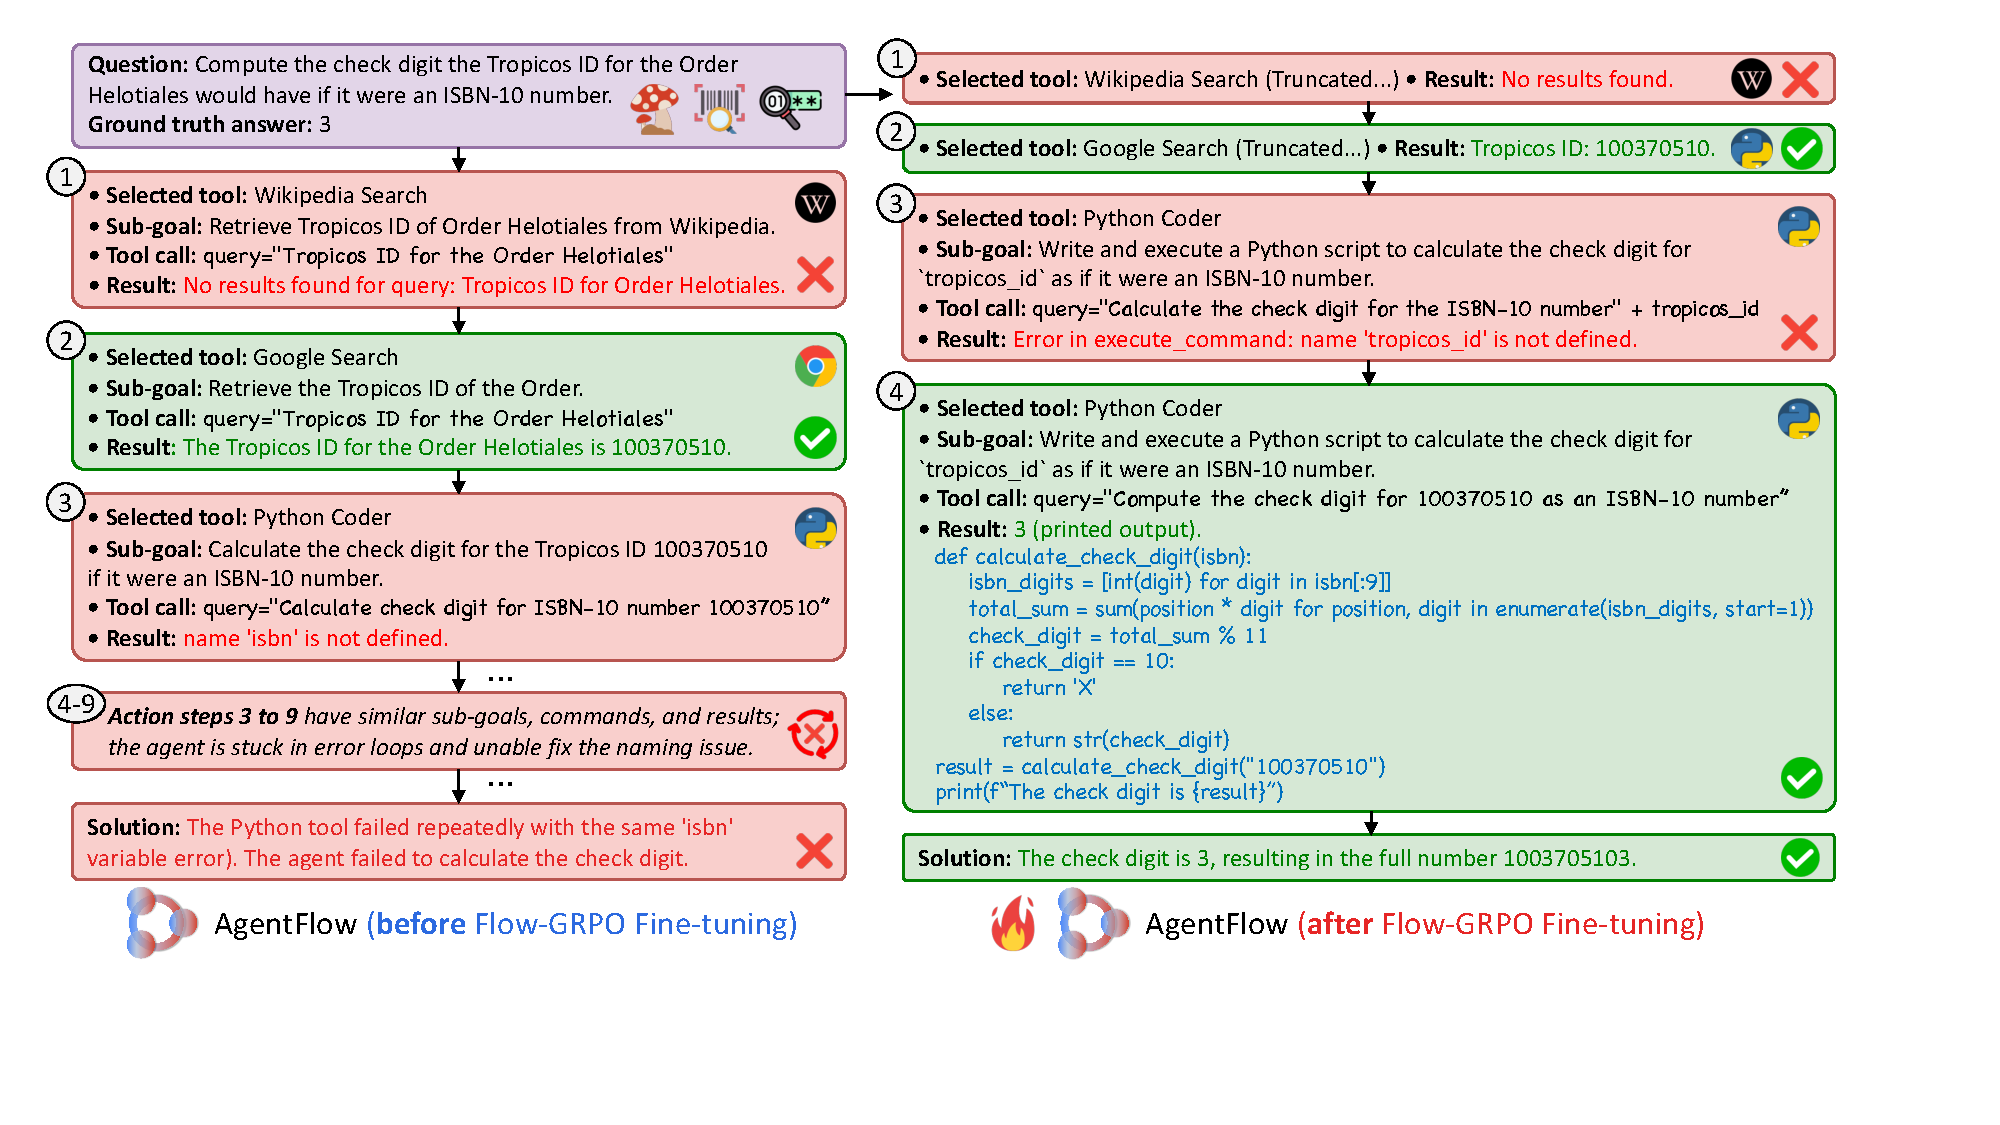
\includegraphics[width=1.0\linewidth]{figs/fig_case_study.pdf}
    \vspace{-6mm}
    \caption{\textbf{One case study example.} Initially failed with repetitive errors (left), \model, trained with Flow-GRPO, explores a new solution pathway at turn 4 after two failed attempts (right).}
    \vspace{-3mm}
    \label{fig:fig_case_study}
\end{figure}


\subsection{Training Strategies on the Planner}
\label{subsec:training_planner}

We conduct an ablation study to analyze the impact of different training strategies for the \textit{Action Planner} module in \model, with results reported in Table~\ref{tab:individual_vs_inflow}. The executor, verifier, and generator modules remain fixed as Qwen2.5-7B-Instruct, consistent with our main setup (\S\ref{subsection:exp_setup}).


\begin{table}[htbp]
  \centering
  \vspace{-2mm}
  \setlength{\tabcolsep}{0.4em}
  \resizebox{0.95\textwidth}{!}{
  \begin{tabular}{llllllllll}
  \toprule
  \textbf{Planner Model} & \textbf{Training} & \textbf{Bamboogle} & \textbf{2Wiki} & \textbf{GAIA} & \textbf{AIME24} & \textbf{AMC23} & \textbf{GameOf24} & \textbf{Avg.} \\
  \midrule
  Qwen-2.5-7B & Frozen & 58.4 & 60.0 & 17.2 & 16.7 & 47.4 & 31.0 & 38.5 \\
  \midrule
  GPT-4o & Frozen & \cellcolor{darkgreen!19.8}65.0 $_{\uparrow~6.6}$ & \cellcolor{darkgreen!30.0}70.0 $_{\uparrow~10.0}$ & \cellcolor{darkgreen!19.2}23.6 $_{\uparrow~6.4}$ & \cellcolor{darkgreen!0.0}16.7 $_{\uparrow~0.0}$ & \cellcolor{darkgreen!3.9}48.7 $_{\uparrow~1.3}$ & \cellcolor{darkgreen!33.0}42.0 $_{\uparrow~11.0}$ & \cellcolor{darkgreen!17.4}44.3 $_{\uparrow~5.8}$ \\
  Qwen-2.5-7B & SFT & \cellcolor{darkred!84.0}30.4 $_{\downarrow~28.0}$ & \cellcolor{darkred!81.9}32.7 $_{\downarrow~27.3}$ & \cellcolor{darkred!32.7}~~6.3 $_{\downarrow~10.9}$ & \cellcolor{darkred!40.2}~~3.3 $_{\downarrow~13.4}$ & \cellcolor{darkred!29.7}37.5 $_{\downarrow~9.9}$ & \cellcolor{darkred!72.0}~~7.0 $_{\downarrow~24.0}$ & \cellcolor{darkred!57.0}19.5 $_{\downarrow~19.0}$ \\
  Qwen-2.5-7B & Flow-GRPO & \cellcolor{darkgreen!33.6}69.6 $_{\uparrow~11.2}$ & \cellcolor{darkgreen!51.6}77.2 $_{\uparrow~17.2}$ & \cellcolor{darkgreen!47.7}33.1 $_{\uparrow~15.9}$ & \cellcolor{darkgreen!69.9}40.0 $_{\uparrow~23.3}$ & \cellcolor{darkgreen!42.3}61.5 $_{\uparrow~14.1}$ & \cellcolor{darkgreen!66.0}53.0 $_{\uparrow~22.0}$ & \cellcolor{darkgreen!51.6}55.7 $_{\uparrow~17.2}$ \\
  \bottomrule
  \end{tabular}
  } %
  \vspace{1mm}
  \caption{Performance comparison of \model across different training methods.}
  \vspace{-2mm}
  \label{tab:individual_vs_inflow}
\end{table}


\textbf{A more capable planner is beneficial, but has limits.} Replacing the frozen \textit{Qwen2.5-7B-Instruct} baseline with a stronger proprietary model, GPT-4o, yields only a modest 5.8\% average gain. This indicates a key bottleneck that, while a more powerful model improves planning, its static nature prevents co-adaptation with the live dynamics of \model.

\textbf{Offline SFT leads to performance collapse, while in-the-flow RL is crucial.} 
The limitations of a static planner are further exposed when distilling GPT-4o's behavior via offline supervised fine-tuning (SFT) on its trajectories as \textit{Action Planner} in \model. This results in a catastrophic performance collapse, with an average accuracy drop of 19.0\% compared to the frozen baseline. 
This failure arises from the token-level imitation objective of SFT, which misaligns with trajectory-level task success and prevents the planner from adapting to dynamic tool feedback or recovering from compounding errors. 
In contrast, training the planner with our on-policy Flow-GRPO method proves highly effective: by optimizing for the final outcome, the planner learns to handle long-horizon workflows, achieving a 17.2\% average gain over the frozen baseline.

\subsection{Scaling Trends in \model}
\label{subsec:scaling_trends}

\paragraph{Training scaling in backbone size.}
We study how backbone LLM scale affects \model's performance and the efficacy of Flow-GRPO. We build two versions of the system: one using \textit{Qwen2.5-3B-Instruct} and another using \textit{Qwen2.5-7B-Instruct} for all four modules (planner, executor, verifier, and generator) and tools. In both, only the planner is fine-tuned with Flow-GRPO. As shown in Figure~\ref{fig:scaling_model_size}, Flow-GRPO fine-tuning consistently improves performance across tasks for both backbones. This demonstrates that our in-the-flow optimization is effective across model capacities, enhancing \model regardless of LLM size.

\begin{figure}[t]
    \centering    
    \begin{minipage}[b]{0.66\textwidth}
        \centering
        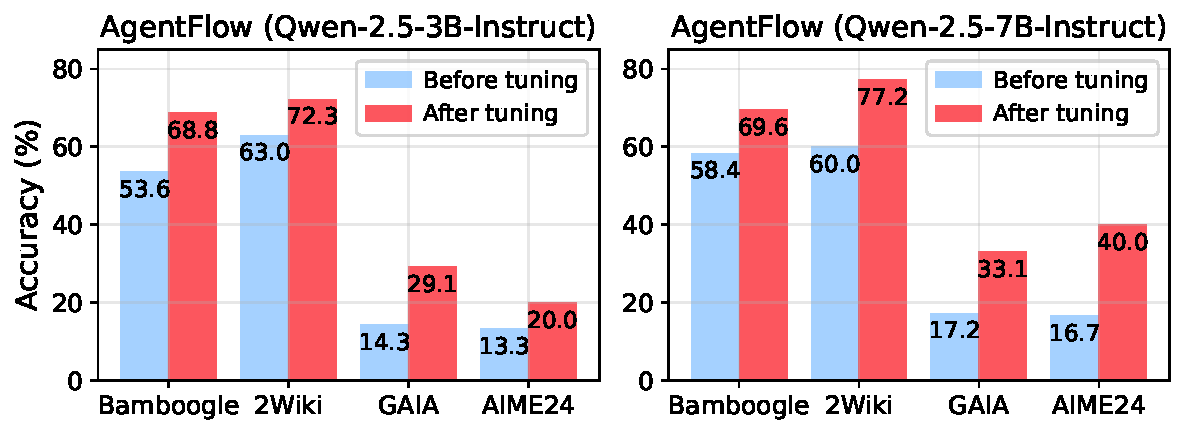
\includegraphics[width=0.95\linewidth]{figs/scaling_model_size.pdf}
        \vspace{-2mm}
        \caption{Flow-GRPO fine-tuning offers consistent gains on \model as the backbone model size scales from 3B to 7B.}
        \label{fig:scaling_model_size}
    \end{minipage}
    \hfill %
    \begin{minipage}[b]{0.32\textwidth}
        \centering
        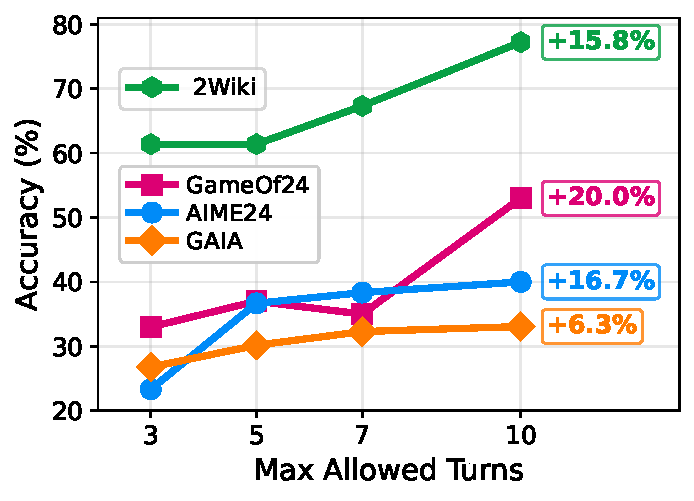
\includegraphics[width=0.95\linewidth]{figs/scaling_turn.pdf}
        \vspace{-2mm}
        \caption{Average accuracy with increased $T_{\text{max}}$.}
        \label{fig:scaling_turn}
    \end{minipage}
    \vspace{-3mm}
\end{figure}

\begin{wraptable}{r}{0.45\textwidth}
    \centering
    \vspace{3pt}
    \footnotesize
    
    \resizebox{\linewidth}{!}{
        \setlength{\tabcolsep}{0.5em}
        \renewcommand{\arraystretch}{0.9}
        \begin{tabular}{lcccc}
            \toprule
            \textbf{Turns ($T_{\text{max}}$)} & \textbf{3} & \textbf{5} & \textbf{7} & \textbf{10} \\
            \midrule
            2Wiki & 2.22 & 3.18 & 3.81 & 4.44 \\
            GameOf24 & 1.63 & 2.12 & 2.36 & 2.67 \\
            AIME24 & 1.63 & 1.63 & 1.86 & 1.90 \\
            GAIA & 2.43 & 3.46 & 4.28 & 5.42 \\
            \bottomrule
        \end{tabular}
    }
    
    \vspace{-2mm} %
    \caption{Average turns with increased $T_{\text{max}}$.}
    \label{tab:scaling_turn} %
    \vspace{-5mm} %
\end{wraptable}

\paragraph{Inference scaling in turn budgets.}
We investigate how the maximum allowed turns ($T_{\text{max}}$) affect reasoning depth and final performance of \model during test-time inference with the Qwen2.5-7B-Instruct backbone. As shown in Figure~\ref{fig:scaling_turn}, increasing $T_{\text{max}}$ from 3 to 10 consistently improves outcomes across all tasks, accompanied by a rise in average turns consumed. On knowledge-intensive benchmarks such as 2Wiki and GAIA, a larger turn budget enables \model for deeper information retrieval. On mathematical benchmarks like GameOf24 and AIME24, it supports decomposed sub-goals, alternative strategies, and refinement of errors. Final performance peaks at $T_{\text{max}}=10$ for all tasks, confirming that a longer reasoning horizon benefits the system without causing degenerate loops. This validates that \model adapts its turn allocation to problem complexity to achieve better solutions through iterative refinement.


\subsection{In-depth Analysis of Optimized Planning}
\label{subsec:optimized_planning}

\begin{wrapfigure}{r}{0.6\textwidth} 
    \centering
    \vspace{-10pt} %
    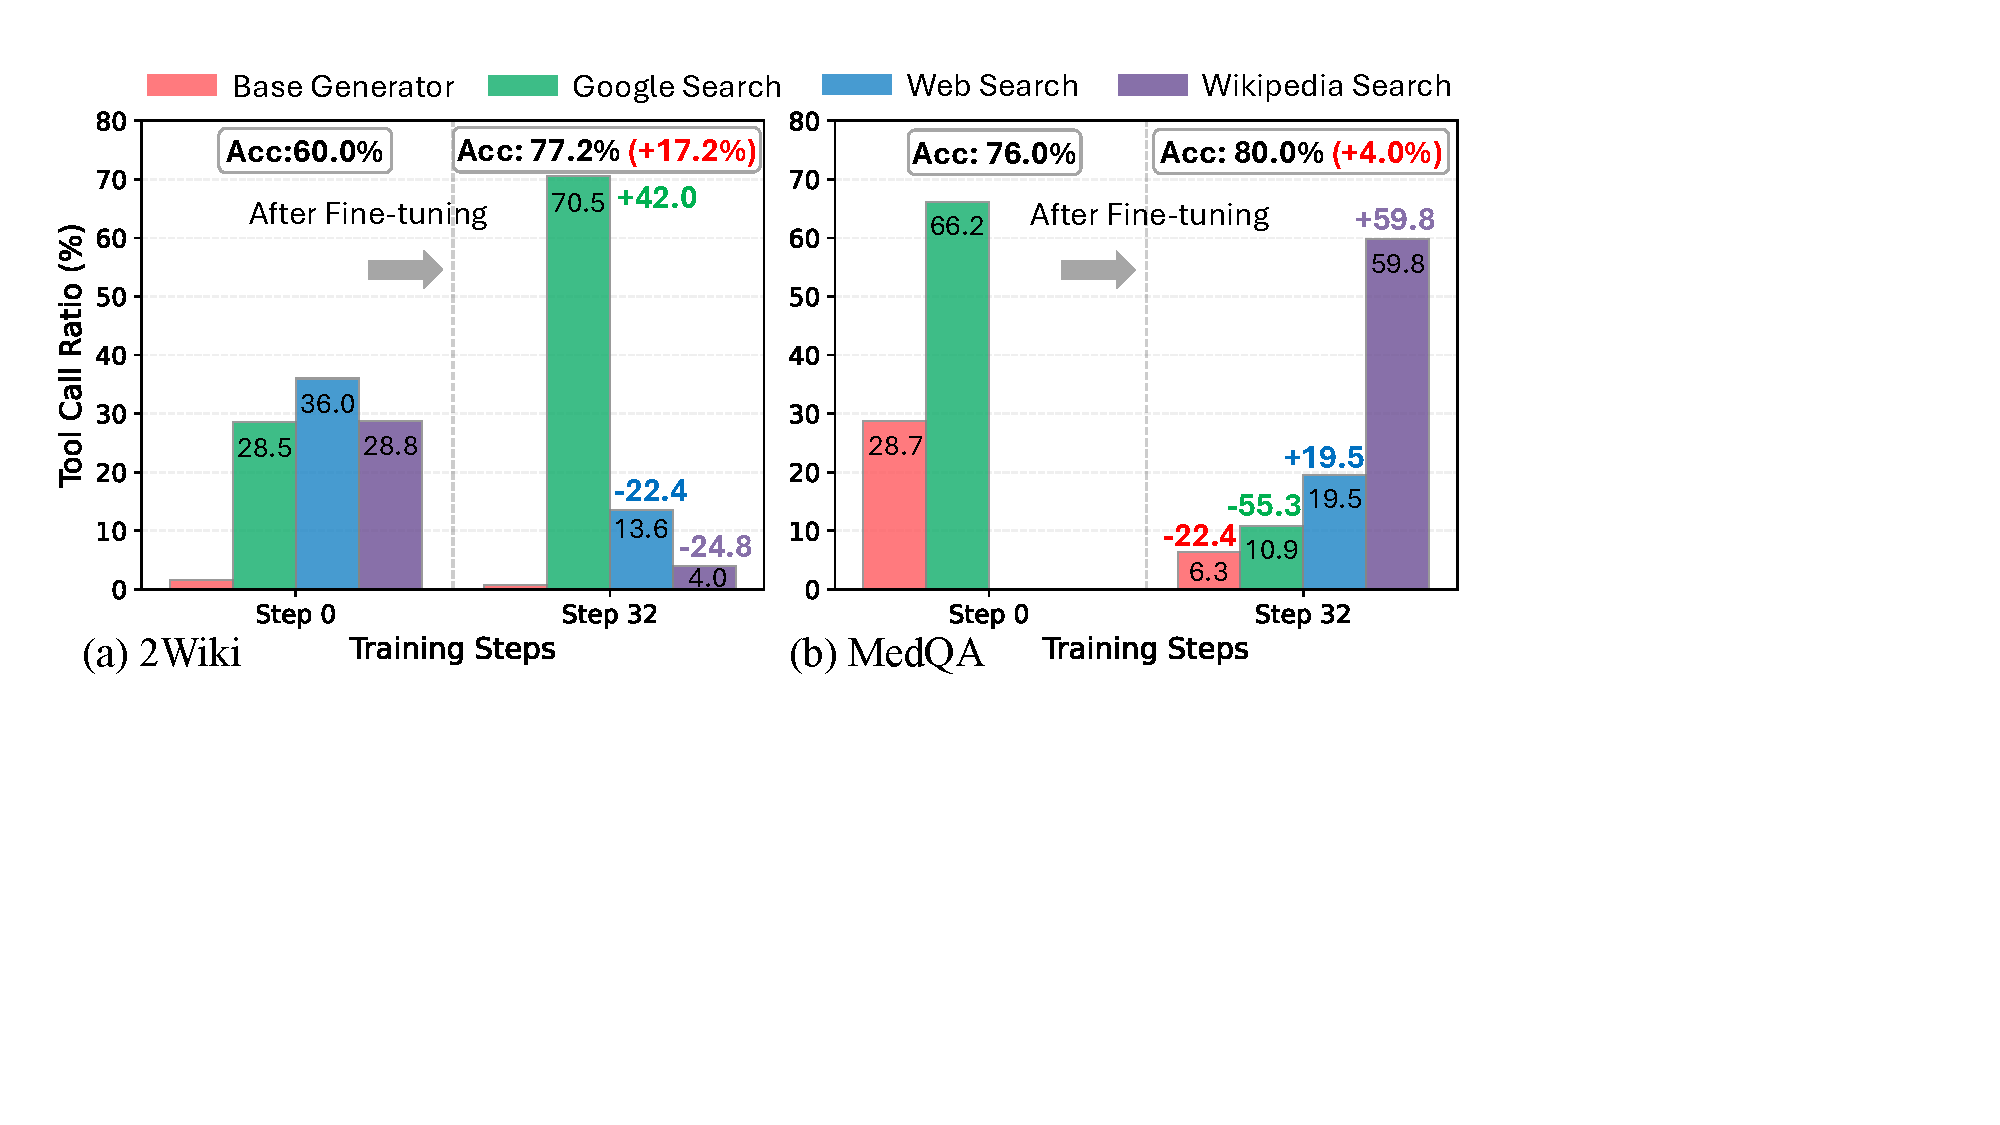
\includegraphics[width=\linewidth]{figs/tool_usage.pdf}
    \vspace{-10pt}
    \caption{Tool call ratio change by Flow-GRPO fine-tuning.}
    \label{fig:tool_usage}
    \vspace{-12pt} %
\end{wrapfigure}

\paragraph{Flow-GRPO optimizes tool usage.} 
We compare tool usage distributions before and after in-the-flow RL training. Figure~\ref{fig:tool_usage} shows results on two knowledge-intensive tasks, 2Wiki and MedQA, which exhibit distinct optimization patterns alongside improved task accuracy. For 2Wiki, which requires broad factual knowledge, Flow-GRPO optimizes the planner to increase Google Search usage by 42.0\%. In contrast, for the specialized MedQA benchmark, which requires deep, domain-specific information retrieval, fine-tuning shifts the planner away from general tools, reducing Google Search calls (66.2$\rightarrow$10.9\%) in favor of in-document Web Search (0$\rightarrow$19.5\%) and specialized  Wikipedia Search (0$\rightarrow$59.8\%). This demonstrates that the planner learns to select task-appropriate tools. 

\paragraph{Flow-GRPO incentivizes autonomous discovery of new solutions.} 
We further examine qualitative examples in Figure~\ref{fig:fig_case_study} and additional cases in \S\ref{app:case_studies}. These cases show that \model, trained with Flow-GRPO, develops enhanced capabilities for task planning and tool use. The planner exhibits adaptive efficiency, stronger self-correction, and spontaneous new integration of tools throughout step-by-step problem-solving, autonomously discovering effective solution pathways.


\vspace{-1mm}
\subsection{Training Efficiency Analysis}
\label{subsec:traing_efficency}


\paragraph{Optimized planning with increased rewards and condensed responses.}
We analyze the training dynamics of the \model planner by tracking its average reward and response length on the train set (Figure~\ref{fig:training_reward}a). Training rewards steadily increase, indicating effective policy improvement via Flow-GRPO. Meanwhile, response length, after an initial exploratory rise, progressively shortens and stabilizes. This shows the planner learns to balance conciseness and informativeness, avoiding unnecessarily long outputs.

\begin{wrapfigure}{r}{0.60\textwidth}
    \centering
    \begin{subfigure}[t]{0.49\linewidth}
    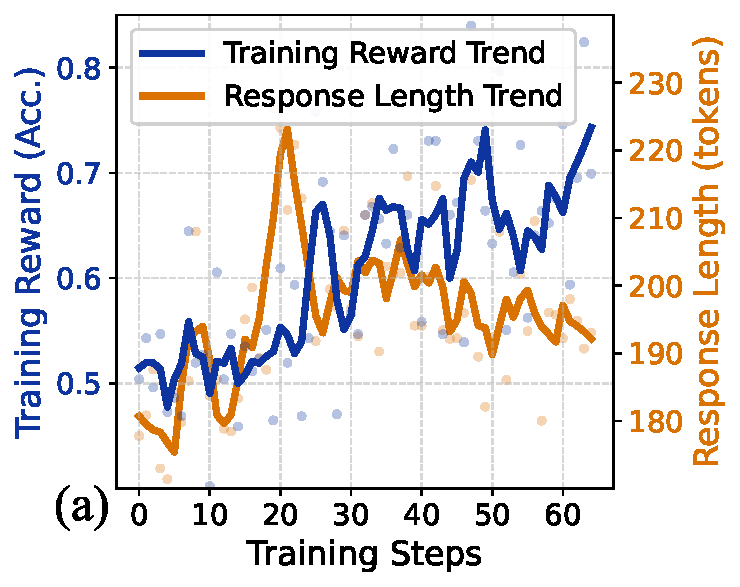
\includegraphics[height=0.15\textheight,keepaspectratio]{figs/train_reward.pdf}
    \end{subfigure}
    \hfill
    \begin{subfigure}[t]{0.45\linewidth}
        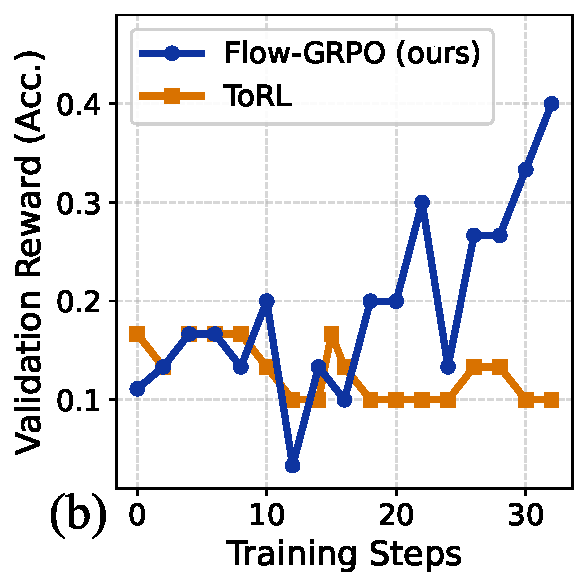
\includegraphics[height=0.15\textheight,keepaspectratio]{figs/val_reward_comp.pdf}
    \end{subfigure}
    \vspace{-2mm}
    \caption{Training dynamics and efficiency of Flow-GRPO.}
    \label{fig:training_reward}
    \vspace{-2mm}
\end{wrapfigure}

\paragraph{Flow-GRPO efficiency over tool-integrated reasoning RL.}
We compare \model (trained with Flow-GRPO) against a monolithic tool-integrated reasoning baseline (ToRL) on AIME24. As shown in Figure~\ref{fig:training_reward}b, \model achieves sustained performance gains, with validation accuracy growing steadily. In contrast, ToRL's performance quickly stagnates and trends downwards, highlighting the superior efficiency of our agentic training approach, which uses decomposition and stable credit assignment to avoid the instability.

\vspace{-1mm}




\vspace{-2mm}
\section{Related Work}
\label{sec:related_work}
\vspace{-1mm}

Reinforcement learning (RL) from outcome-based rewards has become a dominant paradigm for training LLMs to use external tools. Much of this work trains a single, monolithic policy to interleave reasoning with tool calls. This strategy has proven effective in specialized, single-tool settings~\citep{mai2025agent, xue2025simpletir, feng2025retool, li2025torl} and web search for knowledge-intensive questions~\citep{chen2025research, jin2025search, song2025r1, li2025search, sun2025zerosearch}. Recent efforts have extended this monolithic framework to multi-tool environments by focusing on data synthesis \citep{dong2025tool}, unified training infrastructure \citep{jiang2025verltool}, and principled reward design \citep{qian2025toolrl, zhang2025nemotron}. However, these approach scales poorly as task complexity and planning horizons grow. The central challenge is long-horizon credit assignment; attributing a final outcome to specific intermediate tool calls remains difficult, even with fine-grained, turn-level rewards~\citep{zeng2025reinforcing, wang2025stepsearch}. This difficulty leads to training instability and brittle inference-time generalization, manifesting as strategic deficiencies like tool overuse or ``cognitive offloading''~\citep{Wang2025ActingLI, qian2025smart}, suboptimal personalization~\citep{cheng2025toolspectrum}, and poor alignment with user preferences for tool invocation~\citep{huang2025ttpa}.

\paragraph{Agentic systems with tool use.}
Agentic systems offer an alternative to monolithic models by decomposing tasks across specialized modules. Many such systems are training-free, orchestrating pre-trained LLMs with handcrafted logic and prompting, as seen in frameworks like AutoGen~\citep{wu2024autogen}, MetaGPT~\citep{hong2024metagpt}, and OctoTools~\citep{lu2025octotools}. This static approach, however, limits their ability to learn and adapt collaborative strategies from experience. Recognizing this, recent work explores training these systems to improve coordination~\citep{deng2025pe, liao2025marft}. However, most training paradigms are \emph{offline}, relying on supervised fine-tuning or preference optimization on static datasets~\citep{motwani2024malt, park2025maporl}. These methods are decoupled from the live, multi-turn dynamics of the system, preventing modules from learning to adapt to evolving tool outputs or recover from early mistakes. Training directly \emph{in the flow} with on-policy RL is difficult due to sparse rewards and long-horizon credit assignment, where feedback is delayed across long reasoning chains and shifting state distributions~\citep{wang2025ragen}. Consequently, these systems often suffer from brittle adaptation and require complex reward shaping to learn effectively~\citep{wang2025spa}.



\vspace{-2mm}
\section{Conclusion}
\vspace{-1mm}


We presented \model, a trainable, \emph{in-the-flow} agentic system that coordinates four specialized modules via an evolving memory and optimizes its planner directly \emph{inside} the multi-turn loop. To enable stable on-policy learning under long-horizon, sparse-reward settings, we introduced Flow-GRPO, which \emph{converts} multi-turn RL into a sequence of tractable \emph{single-turn} policy updates by \emph{broadcasting} a single, verifiable trajectory-level outcome to every turn and stabilizing credit assignment with group-normalized advantages. Comprehensive experiments show that \model achieves strong cross-domain performance, surpassing specialized baselines and even larger proprietary models. In-depth analyses confirm improved planning and tool-calling reliability, along with positive scaling trends in model size and allowed turn budgets.

\section*{Acknowledgment}
We would like to thank Yihe Deng, Xuehang Guo, and Kunlun Zhu for their valuable input during the early stages of this work. We are also grateful to Lambda for providing GPU resources. This work was partially supported by the Hoffman-Yee Research Grants program at Stanford HAI, the AI for Math Fund by Renaissance Philanthropy, ONR MURI N00014-24-1-2748, and the AI Research Hub Project through KAIST. This work was also supported by IITP (No.~RS-2024-00457882, National AI Research Lab Project).
